% This file is isea.tex.  It contains the formatting instructions for and acts as a template for submissions to ISEA 2015.  It is based on the ICCC  formats and instructions.  It uses the files isea.sty, isea.bst and isea.bib, the first two of which also borrow from AAAI IJCAI formats and instructions.
% Modified from ICCC.tex by B. Bogart

\documentclass[letterpaper]{article}
\usepackage{isea}
\usepackage[pdftex]{graphicx}
\usepackage{times}
\usepackage{helvet}
\usepackage{courier}
\usepackage{url}
\usepackage{verbatim}
\usepackage[numbers]{natbib}
\pdfinfo{
/Title Extend segment routing for another source routing protocol named RPL for Linux
/Author Alexander Aring, Stefan Schmidt, Michael Richardson}
% The file isea.sty is the style file for ISEA 2015 proceedings.
%
\title{Extend segment routing for another source routing protocol named RPL for Linux}
\author{Alexander Aring, Stefan Schmidt, Michael Richardson\\
Unemployed Hobbyist, Open Source Developer, Sandelman Software Works\\
Ottawa, Canada/Brunswick, Germany\\
alex.aring@gmail.com, stefan@datenfreihafen.org, mcr@sandelman.ca\\
\newline
\newline
}
\setcounter{secnumdepth}{0}

\begin{document}
\maketitle
\begin{abstract}
RPL \cite{RFC6550} is an IPv6 routing protocol for Low-Power and Lossy networks with interesting use cases in the IoT domain.

There exists many different open source RPL implementations for Linux, which are using RPL with storing mode only.
In storing mode the routes are propagated via ICMPv6 RPL messages and stored inside the routing table of the Linux kernel.
In contrast, the non-storing mode is using source routing by adding header information \cite{RFC6554}.

This paper is about our work to implement RPL non-storing mode source routing for the Linux
kernel and offer the necessary configuration interfaces to user space.
We implemented rpld \cite{rpld} to show an example RPL implementation which will
make use of the configuration interfaces to support non-storing mode.
As reference we will lookup the Linux segment routing implementation and try to extend the existing code.
Initial discussion about the approach choosen have been discussed during Netdevconf 2.1.
\end{abstract}

\section{Keywords}

Linux, IPv6, Low-Power and Lossy Networks, LLN, IPv6 Routing Protocol for Low-Power and Lossy Networks, RPL, Segment Routing, Source Routing

\section{Introduction}

With storing and non-storing RPL offer two different operations modes.
Before we can go into the details of the implementation in this paper, this section will explain the differences between these modes.
We will describe how RPL generates routes based on an example mesh topology.
As RPL generates a tree like routing graph there exists upward routes as a route to the root node and downward routes as a route to child nodes.

\subsection{Topology}

In this paper we simplify RPL routing graph as a tree like structure with one parent and a list of children named DODAG (Destination-Oriented Directed Acyclic Graph).
Out of scope are other topologies e.g. multiple roots or floating roots, where the root node can be changed during runtime.
We want to keep the topology simple enough to first tackle the issue of non-storing mode inside GNU/Linux environment.

RPL avoids to use the IPv6 neighbor discovery. All nexthop destination will use link-local addresses which are setup by stateless autoconfiguration.
In order to get basic RPL configuration the network is flooded with a DIO (DODAG Information Object) message.

\subsection{Upward Routes}

Each node, except the root node (DODAG root), maintains upward routes.
In both operation modes the upwards routes are stored inside the routing table.
This nexthop address is declared as parent (DODAG parent), because in view of
the actual node the root can be reached over its parent and traversing the tree further up.
All unknown destination addresses will be routed to the parent which finally reach the root node.
The root can act then as a RPL Border Routing and route packets to a different IPv6 network.

\paragraph{Parent Selection}

In case of multiple possible parents RPL provide mechanism for parent selection.
One which considered all parent selection up to the root node is MRHOF \cite{RFC6719}.
MRHOF considers the link quality between the node and their parents.
However this is out of scope of this document as basic parent selection can be considered a first come, first serve strategy when a DIO message arrived.

\subsection{Downward Routes}

In downward routes the operation mode can be different.
Downward routes are neededto reach child nodes until leaf nodes from any parent or the root.
As mentioned earlier the operation mode can be storing or non-storing mode.
In this section we describe the difference of both operation modes.

\paragraph{Storing Mode}

In storing mode the downward routes are stored in {\bf all} nodes inside the routing table in their IPv6 stack instance like the upward routes.
Each nodes reports to his parent, decided before during parent selection, his reachable nodes over his children.
Therefore a DAO (Destination Advertisement Object) message will be send to the parent which contains all child nodes.
For this very reason a DAO contains multiple RPL Target Options which contains each global-link address reached by specific link-local child address.
Starting from the leaf, each node will report it's parent their children and add their own address.

As result each nodes maintains a routing table in its IPv6 stack instance how every child in view of a specific node can be reached.
If the destination address isn't specified in the routing table, the default route will route the packet to the root node.
No source routing is involved, the forwarding inside this RPL operation mode is handled by looking up the forwarding table only.

\paragraph{Non-Storing Mode}

In non-storing mode the nodes doesn't store any forwarding table information except one route for upward routes.
This has the effect that all packets will be routed to the root node of the network.
The root node will take use of source routing and adds, if the destination address is part of the RPL network, a RPL source routing header as IPv6 extension header.
This source routing header has every nexthop to reach the final destination node inside the RPL network.
A RPL node sends for this case the DAO message not to it's parent, it will be directly routed to the root node.
Such DAO message will contain two options, the node node global-link address and it's parent link-local address.
The root node has a full topology overview of the RPL network and can reconstruct the segment link-local addresses to reach a specific child node.

\section{Example}

This section describes an example topology to show the information described in the previous sections.

\subsection{Topology}

\begin{figure}[h]
	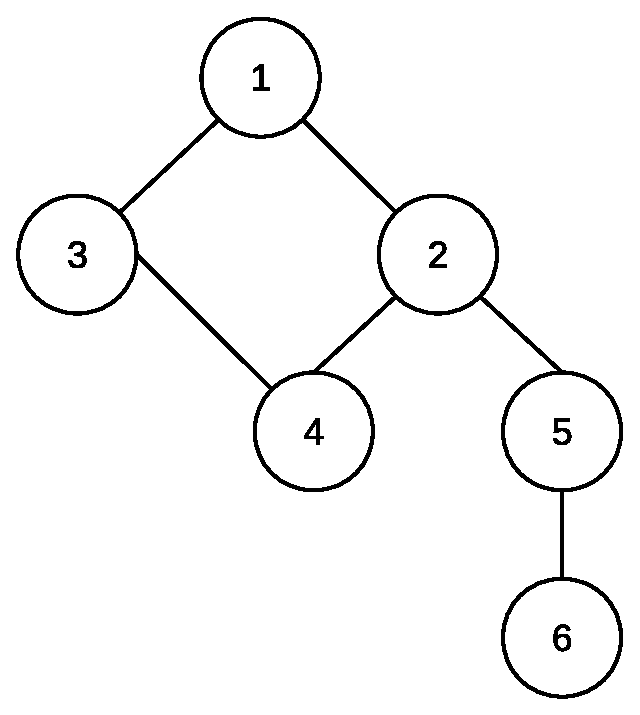
\includegraphics[width=3.31in]{figs/mesh0.eps}
	\caption{Example mesh topology with bidirectional edges}
	\label{mesh0}
\end{figure}

\subsection{RPL DODAG}

\begin{figure}[h]
	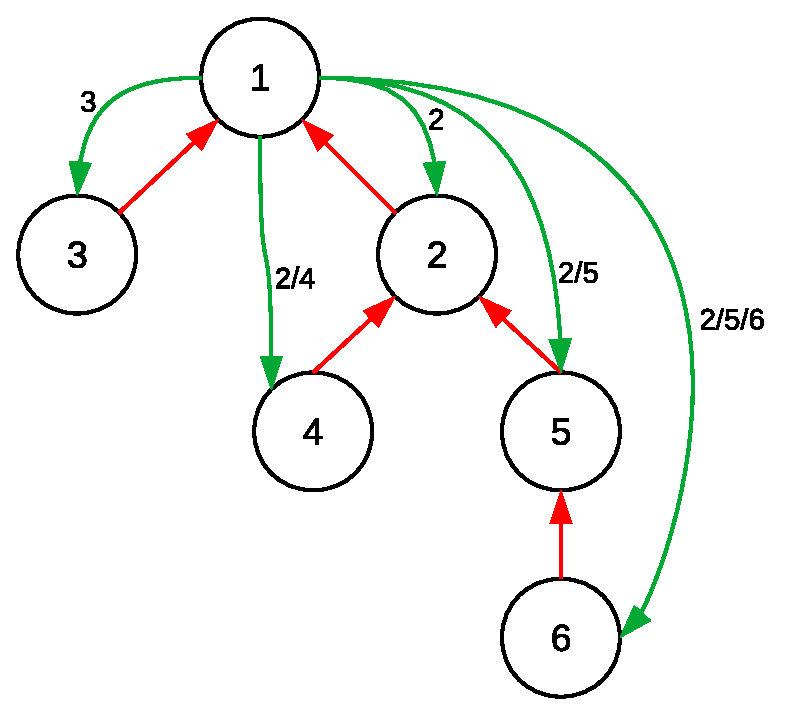
\includegraphics[width=3.31in]{figs/mesh1.eps}
	\caption{Resulting RPL topology in ``non-storing`` mode of mesh topology as shown in figure \ref{mesh0}}
	\label{mesh1}
\end{figure}

In Figure \ref{mesh0} we show an example mesh topology. In this example the
edges are bidirectional, and every node can reach every other node. Following on
in figure \ref{mesh1} we show a possible resulting RPL DODAG of the mesh topology from figure \ref{mesh0}.
Upward routes are shown as red directional arrows to reach the root node which was set by parent selection.
The root node stores a configuration to setup downward routes shown as green arrows.
These downward routes will be added as source routing header to the IPv6 header.
The children of the RPL network will actually not store any downward routes information and get the forwarding information from the routing header.
These forwarding information are shown beside the green arrows with node number and a separation character.
For example the root node can reach the child node 6 via node 2 over 5 to 6.

\section{Analysis}

When writing this document current RPL implementations for Linux, like rpld or
unstrung \cite{unstrung}, are supporting storing mode only.
The main blokcer for implementing non-storing mode in a routing deamon are some
unsolved issues we will describe in the problem subsection. We describe the
problem in Linux, which need to be solved to provide non-storing mode.
Afterwards multiple possible solutions will be evaluated and the decision fo our
approach explained.

\subsection{Problem}

The problem user space routing implementations face is IPv6 header generation is
happening inside in kernel space on Linux.
As the RPL source routing header is an extension header of IPv6 header, it need to be added inside the kernel transmit path of the IPv6 stack.
The current state of Linux kernel has no implementation to insert these headers to the IPv6 header.
Storing mode is not effected by this as it does not use this technique. For
non-storing mode it has been a blocker for most RPL implementations.

On the receiving path, the IPv6 stack need to parse the RPL source header information and forward it to the nexthop if necessary.

\subsection{Requirements}

The root node of the RPL DODAG (DODAG root) needs to have the possibility to insert a RPL source header with specific configurations per destination address.
This is necessary when a IPv6 packet from a child arrived over it's parent path
and needs to be forwarded to another known child of the RPL network which only the root node knows.
If a root wants to send a packet to a known child the RPL source route header
needs to be attached with the right path information to it's child as well.

{\bf Each node} needs to handle the RPL source routing header by parsing the header and handle forwarding of this packet to the nexthop correctly as RFC6554 describes.
This needs to be done in the Linux IPv6 forwarding plane and not after.

\subsection{Socket Option}

There exists the possibility to add a specific source route header over the socket option ``IPV6\_RTHDR`` in Linux.
This can be used to place a RPL source routing header per IPv6 on a per socket setup.
It can also be used to send out IPv6 packets with a specific RPL source header without getting the kernel involved of placing a source routing header.

The socket option can not be used to implement a solution that meets the
requirements to add a specific source routing header for a specific destination
address, as it is only used inside the per socket context.
It also can not handle the parsing of IPv6 packets and forwarding them by not reaching the Linux socket layer.

\subsection{Lightweight Tunnel}

A lightweight tunnel (lwtunnel) in Linux can be used to meet the requirement of
generating RPL source route headers for a specific destination.
Therefore we can lookup the implementation of IPv6 segment routing \cite{srh} of the Linux kernel implementation.
Lightweight tunnels can be registered over a ops structure inside the Linux kernel.
For per route destination, which is in RPL only a full IPv6 address and not a prefix
route, an encapsulation type can be given to assign the route to a specific lwtunnel.
Incoming and internal packets for a specific destination lwtunnel will be encapsulated by a RPL source routing header with a specific configuration given by the lwtunnel at creation time.

There is still an open requirement of parsing and forwarding packets which will be discussed in the next section.

\subsection{Forwarding}

This section describes a solution how to parse and forward a IPv6 packet with a RPL source routing header.
The following approach is identical to how IPv6 segment routing \cite{srh} is solving the same requirement.

In this approach the source routing header handling and forwarding is just placed into the next header handling of the IPv6 stack.

\subsection{eBPF}

The Linux kernel has eBPF hooks for the lwtunnel implementation.
This means that the generation of RPL source route header can be implemented as a lwtunnel in eBPF.

On the other hand there exists no eBPF hooks for the forwarding requirement which also requires to parse the header and interact with the IPv6 forwarding handling.

\subsection{Decision}

After evaluating all possible options to implement the requirements we found
that the socket option doesn't meet the requirements and the eBPF handling requires new hooks and for the lwtunnel additional user space handling to make it work.
The conclusion is to provide an in kernel lwtunnel implementation and extend the IPv6 extension header parsing with handling for RFC6554 RPL source routing header.

\section{Design}

This section describes the design for the upcoming implementation part.
It contains the explanation of the user view how to use the RPL source routing functionality.
This contains handling of the sysfs and netlink interfaces and also has a side
note on the compression functionality of the RPL source routing.

\subsection{Sysfs}

The segment routing implementation for processing of RPL source routing headers
will be disabled by default. The sysfs interface for IPv6 configuration will be
extended to allow enabling the processing of these headers.

\subsection{Compression}

The RPL source routing header of RFC6554 can be in a compressed format.
According to the IPv6 destination address the same prefix bytes can be elided.
The compression implementation follows a simple design of providing compress and uncompress functionality.
Any provided format can be converted into a different format according to the destination address context information.

In some cases it's necessary to change source routing header information which
may available in a compressed format only. To avoid mistakes in the
implementation the common approach is to handle such changes as following:

\begin{enumerate}
\item{Uncompress RPL source routing header}
\item{Change RPL source routing header information}
\item{Compress RPL source routing header again}
\end{enumerate}

This provides a simple modification of the segment addresses as these are available in a non-compressed format.

\subsection{Linux Kernel Netlink}

The Netlink API for the RPL source routing should align itself with the same API
principles of the existing segment routing implementation.
The segment routing API is designed to provide the source routing header as binary data according to an IPv6 routing prefix.
For simplification of API the routing header will be accepted only in a uncompressed format.
This simplification has the benefit of avoided cases where the routing prefix is
giving as non full address and the final destination address is available at runtime only.
We have one exception, if the routing prefix is a full IPv6 address prefix, which can avoid a compression during runtime.

\subsection{rpld}

The RPL daemon exchange ICMPv6 messages to setup necessary routing information.
At the state of writing this paper the RPL daemon already supports storing mode
by using this functionality.
When the rpld daemon is starting it will setup the necessary sysfs entry settings to allow the forwarding of RPL source routing headers.
The RPL daemon will be extended to support non-storing mode by introducing a new configuration option named ``mode-of-operation``.
RFC 6550 describes ``mode-of-operation`` as a byte parameter for broadcasting routing protocol parameters through the network.
The root node of the RPL will initial flooding the network with these
parameters, inclusive the global-link IPv6 address.
When other nodes receiving these parameters they will be preparing their upward
routes by executing parent selection.
Over the upward routes the nodes will send their parent and own global-link
addresses to the root node of the RPL network.
The RPL root node constructs the RPL topology and configures the downward routes to each node by using the RPL source routing Netlink API.

\subsection{iproute2}

The iproute2 design follows all other lightweight tunnel mechanisms.
This functionality is not necessary for the rpld daemon to work, but it is a different configuration tool to show or manipulate the current RPL source routing settings.

\section{Implementation}

This section describes the implementation of our design. It contains the
necessary changes inside the Linux kernel and user space software which where needed to implement RPL in ``non-storing`` mode.

\subsection{Linux kernel}

The Linux kernel will be extended to forward and generate RPL source routing
headers to an Linux IPv6 stack generated IPv6 packet.

\paragraph{Compression Helpers}

To provide RPL compression and decompression functionality the file ``net/ipv6/rpl.c`` was introduced.
This will be always build with the Linux IPv6 stack implementation to allow
handling RPL source routing headers during runtime.
This is part of the forwarding handling.

The API of the helper functionality is defined as follows:

\begin{itemize}
	\item{size\_t ipv6\_rpl\_srh\_alloc\_size(unsigned char n)}
	\item{size\_t ipv6\_rpl\_srh\_size(unsigned char n, unsigned char cmpri, unsigned char cmpre)}
	\item{void ipv6\_rpl\_srh\_decompress(struct ipv6\_rpl\_sr\_hdr *outhdr, const struct ipv6\_rpl\_sr\_hdr *inhdr, const struct in6\_addr *daddr, unsigned char n)}
	\item{void ipv6\_rpl\_srh\_compress(struct ipv6\_rpl\_sr\_hdr *outhdr, const struct ipv6\_rpl\_sr\_hdr *inhdr, const struct in6\_addr *daddr, unsigned char n)}
\end{itemize}

There are two size calculation methods, ``ipv6\_rpl\_srh\_alloc\_size()`` should
be used to get the allocation size to decompress the RPL header.
This function will allocate worst case memory size for segments area according to n segments.
On the other hand ``ipv6\_rpl\_srh\_size()`` will return the size of a compressed header according to the number of n segments and RPL specific parameters ``cmpri`` and ``cmpre``.
This function can be used to validate a RPL header before dereferencing it to
potential buffer overflows.

The necessary parameters used in the helpers are described as following:

\begin{description}
	\item[cmpri]{The amount of prefix bytes of the segment addresses (except last one) which are the same of the actual used IPv6 destination address}
	\item[cmpre]{The amount of prefix bytes of the last segment address which are the same of the actual used IPv6 destination address}
	\item[n]{Number of segments inside the segment header, can be calculated by cmpri and cmpre}
	\item[outhdr]{Destination buffer for the compression or decompression of RPL header}
	\item[inhdr]{Source buffer for the compression or decompression of RPL header}
\end{description}

\paragraph{Forwarding}

The forwarding implementation is in the Linux kernel file
``net/ipv6/exthdrs.c``, which is always build.
As base implementation, most code was re-used from the IPv6 segment routing implementation.
RPL source routing processing mechanism requires additionally handling at some points.

Similar to segment routing the IPv6 destination address need to be swapped with the segment address one, pointed out by the ``segment\_left`` field of the RPL source routing header.
To do this manipulation we do a three step decompression, manipulation and
compression  procedure.
As the header size can result in different sizes before and afterwards, a full skb\_pull() of the extension header is necessary.

Another requirement is to detect possible loops in the address segments.
It needs to be checked that a non assigned IPv6 address on the forwarding route appears separate inside the segments array.
The implementation of this functionality can be found as ``int ipv6\_chk\_rpl\_srh\_loop(struct net *net, const struct in6\_addr *segs, unsigned char nsegs)`` inside ``net/ipv6/addrconf.c``.
This helper functionality returns one if any address occurs separated inside the segmented array, otherwise it will return zero.
The packet will dropped and a special ICMPv6 error messages will be generated as RFC 6554 descibes.

\paragraph{Lightweight Tunnel}

To generate IPv6 packets with a RPL source routing header in Linux a lightweight tunnel implementation was introduced.
This feature can be disabled or enabled during compile time with the ``IPV6\_RPL\_LWTUNNEL`` config entry.
The implementation of this functionality can be found in ``net/ipv6/rpl\_iptunnel.c``.

The initial code handles only inline extension header and no IP encapsulation.
Although IP encapsulation is handled in the forwarding code the current RPL lwtunnel implementation doesn't support to generate such packets.
Currently the ROLL working group tries to summary the requirements for IP
encapsulation in a different draft \cite{I-D.ietf-roll-useofrplinfo}.

\subsection{iproute2}

The iproute2 implementation contains two basic methods to create a routing
configuration to add a RPL source routing header for a specific IPv6 destination address.
Therefore the specific segments are needed to be given on the command line.
Additionally the current configuration can be dumped via iproute2.
The parsing and printing from and to command line can be shared between IPv6 segment routing and RPL segment routing code.
As indicator to specify a RPL source routing lwtunnel configuration the keyword ``rpl`` will be used.

Example: ``ip -n ns0 -6 route add 2001::3 encap rpl segs fe80::c8fe:beef:cafe:cafe,fe80::c8fe:beef:cafe:beef dev lowpan0``

\subsection{rpld}

To implement ``non-storing`` mode a tree data structure is required to represent the current RPL topology inside the root node.
A basic implementation with key value pairs of the global-link address and their link-local address was added to the rpld implementation.
If a DAO messages arrived the source global-link address will be used to store the node into the tree according to it's parent from the parent selection algorithm.
Storing a node inside the topology will lead ta a Netlink message being send to the kernel to setup a RPL source route.
With such a mechanism every node reports to the root node their parent and own address, the root node can calculate the path from the root to it's child and construct the necessary segments setup from the taken path.

\section{Testing}

In this section we describe how we tested the implementation and confirmed that it's actual working.

\subsection{mac802154\_hwsim}

For our testing we used mac802154\_hwsim driver to create virtual IEEE 802.15.4
devices in Linux and constructed a mesh topology.
At the end we had several IPv6 capable interfaces separated in their net namespace in a specific topology.

\subsection{wireshark}

Wireshark \cite{wireshark} was used to capture traffic on the IPv6 interface to confirm the RPL source router header was inserted.
At writing of this paper Wireshark was capable to dissect the RPL source routing header so it was easy to verify the compression algorithm to work correctly regarding to the Wireshark implementation.

\subsection{iputils}

Finally iputils \cite{iputils} was used for ping and traceroute to confirm that every node was addressable.
Traceroute was showing the upward and downward routes correctly, that the traffic inside the RPL network was going always over the root node.

\section{Future Work}

This paper shows how the basic RPL segment routing is implemented for the Linux kernel.
There remains future work to optimize the performance and adding new features, in this are which we layout in this section.

\subsection{Tweaks}

Currently the uncompressed RPL header is set by using the Netlink API.
The RPL header gets decompressed during runtime when the full IPv6 destination address is known.
This could be optimized for cases where the lwtunnel routing prefix is in a form
of a full IPv6 destination address. In this scenario we can do a compression at
configuration time and can save the compression algorithm run during runtime in
a hotpath. Having a full address routing prefix is a common thing in the RPL routing protocol.

\subsection{IP encapsulation}

As mentioned before, the creation of IP encapsulation for RPL lwtunnels is not supported yet.
The only supported mode is inline. The ROLL IETF working group works on defining
the cases when IP encapsulation \cite{I-D.ietf-roll-useofrplinfo} can or should
be used.
However, this is not necessary to get RPL source routing running in a controlled network.
In cases of several RPL networks are interconnected through the internet IP encapsulation may be required.

\subsection{Mixed Mode}

Michael Richardson pointed out that the ROLL IETF working group is working on a
mixed mode of ``storing`` and ``non-storing`` modes.
As ``non-storing`` mode routes every traffic over the RPL root in can happen that direct downward routes can be shorter.
This feature doesn't require any change to the Linux RPL kernel functionality, but RPL routing daemons like rpld need to be updated to set routes differently.

\section{Bugs}

This section describes bugs which we detected while implementing and using the showed approach for RPL source routing for Linux.

\subsection{IPv6 Segment Routing}

When implementing the lwtunnel we figured out that in ``struct lwtunnel\_state`` a field named ``headroom`` which was set inside the IPv6 segment routing implementation.
As we adapted the code base from the IPv6 segment routing implementation as
well, we figured out that setting this value with an IPv6 minimum MTU size
interface causes problems. Researching this showed that this field was introduced by the MPLS lightweight tunnel which operates before the IP layer.
As the Linux interface MTU is layer 3, this headroom value specifies the additional amount which is required before IPv6 such as MPLS.
In out environment, on an IPv6 minimum MTU interface, the IPv6 segment routing ``sendmsg()`` call will return an error.
There is still a discussion going on what the ``headroom`` value really means. As it breaks 6LoWPAN interface for the RPL lwtunnel implementation it is set to zero.

\subsection{iputils - Traceroute}

When we started to use traceroute to test our implementation it was not working
correctly. After debugging the comunication with Wireshark it was found that the
implementation is not dealing with the next header chain of IPv6 correctly.
A quick fix was prepared and a problem description was send to iputils
developers as pull-request \cite{iputilspr}. However Michael Richardson pointed out that handling next headers correctly has it's own RFC \cite{RFC7045}.
Preparing a clean solution for this problem  is still pending as future work.
Currently it is just not working for RPL source routing extension headers.

\bibliographystyle{isea}
\bibliography{isea}

\end{document}
